\documentclass{ltjsbook}
\usepackage{docmute} 
\usepackage{../../myStyle} 

\begin{document}
\setcounter{chapter}{8}
\chapter{システム論からみた社会心理学;第二，第三世代システム}
\label{sp09_system}

\section{Belousov–Zhabotinsky反応}

まずは今日はちょっと変なものから見てもらおうと思います。変なものとは言わないんですけど，はい，これです。ちょっと見てくださいね\footnote{講義中は動画を投影していました。}。
\begin{figure}[ht]
	\centering
	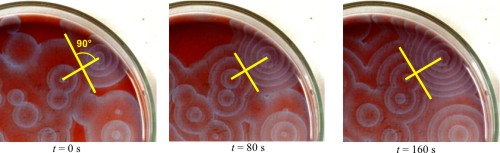
\includegraphics[keepaspectratio,width=0.7\linewidth]{../images/09_BZ.jpg}
	\caption{Belousov–Zhabotinsky反応の例(Wikipediaより。ドイツ語版ウィキペディアのJkriegerさん - de.wikipedia からコモンズに移動されました。
    パブリック・ドメイン, \url{https://commons.wikimedia.org/w/index.php?curid=2794047}による)}
	\label{BZ}
\end{figure}

このピペットの中にあるものを棒で突くとですね，こういうモワーっとした模様が内側から次々に現れてくるというやつです。ご存知ですか？これはBelousov–Zhabotinsky反応\footnote{ベロウソフ・ジャボチンスキー反応(ベロウソフ・ジャボチンスキーはんのう，英: Belousov–Zhabotinsky reaction，略してBZ反応\index[termidx]{びーぜっとはんのう@BZ反応}とも呼ばれる)とは，セリウム塩などの金属塩と臭化物イオンを触媒としてマロン酸などのカルボン酸を臭素酸塩によりブロモ化する化学反応のことである。系内に存在するいくつかの物質の濃度が周期的に変化する非線型的振動反応の代表的な例として知られている。(Wikipediaより)}と言われるやつで，美しい化学反応として知られています。これは僕がどこかで見つけた画像なので，BZ反応\index[termidx]{びーぜっとはんのう@BZ反応}とかで調べてもらうと，こういった動画がウェブとかから検索で出てくるかと思いますので，見てみてください。

この次々と，内側から次へ次へと，何か丸い模様が反応して繰り返し出て来る様子がいいですね。拡張する境界が他の境界と接触すると，内側から広がっていくなどして，次々と拡大していく模様が見えるかと思います。これはこんな感じの美しい反応という話で，社会心理学\index[termidx]{しゃかいしんりがく@社会心理学}の授業なのにこれを見せてどうするんだ，何を思えというのだ，と思われるかもしれませんが，これが今日お話しするシステム論\index[termidx]{しすてむろん@システム論}の第二世代に関わるところですので，最初ちょっと映像としてお見せしたような次第です。

さて，この話はこれぐらいにしておいて，全体で言うと9回目なんですが，システム論\index[termidx]{しすてむろん@システム論}の第二回目の講義を始めていきたいと思います。

\section{第二世代システム}

\subsection{前回の授業の振り返り}

前回から，システム論\index[termidx]{しすてむろん@システム論}から見た社会心理学\index[termidx]{しゃかいしんりがく@社会心理学}というような話で進めています。前回，第一世代システム\index[termidx]{だいいちせだいしすてむ@第一世代システム}という話をしました。第一世代システム\index[termidx]{だいいちせだいしすてむ@第一世代システム}のサブタイトルは動的平衡系\index[termidx]{どうてきへいこうけい@動的平衡系}。インプットとアウトプットを繰り返しながら安定状態を保つという，ダイナミックに安定している系についての記述を扱いました。

生物の話を考えるときは，ホメオスタシス\index[termidx]{ほめおすたしす@ホメオスタシス}(恒常性)と言われるように，生物の状態を一定の状態にしておこうというシステムはあちこちに見かけられるわけでして，こういったものの見方を一般論として語りましょうというのが，一般システム理論\index[termidx]{いっぱんしすてむりろん@一般システム理論}General System Theoryです。ベルタランフィー\index[nameidx]{べるたらんふぃー@ベルタランフィー}が目指していたところはそういうところだったわけです。

ベルタランフィー\index[nameidx]{べるたらんふぃー@ベルタランフィー}の話は，そもそもダイナミックな中で安定するシステムという話でしたから，それをジェネラルにしたいというのが目標としてありました。そこで彼はシステムを，連立微分方程式\index[termidx]{れんりつびぶんほうていしき@連立微分方程式}の形で書いたわけですね。ベルタランフィー\index[nameidx]{べるたらんふぃー@ベルタランフィー}がそれを唱え始めた頃というのは，連立微分方程式\index[termidx]{れんりつびぶんほうていしき@連立微分方程式}にすると，かろうじて解のパターンが分類分けできるという時代でした。ダイナミックなシステムというのを語る上でそういった定式化をして，特に要素の$Q$に当たるところを限定しないで議論することによって，様々な現象に対応できるんだというのが，第一世代システム\index[termidx]{だいいちせだいしすてむ@第一世代システム}のスタートでした。

そもそも第一世代として，システムという考え方が出てきた一番の理由は，生命というのを考えたいんだというところにあったんですね。このモチベーションのところを押さえておいていただくと，この学問体系の目指すところがイメージしやすいかと思います。


さて，前回の授業に対するコメントをいただきました。コメントには，生物系の授業を取っていたときに入出力のシステムとして考え方が出てきたという，ご意見をいただきました。私は前回，「システム論\index[termidx]{しすてむろん@システム論}をどこで教えているのかな」と言いましたが，生物系の話で触れられるんですね。あるいは今日，うちの院生に聞いてみたのですが，人工生命の学会に行ったときに聞いて知った，ということでした。体系的に教えられているかどうかは分かりませんが，生命を考えるというときにこのシステム論\index[termidx]{しすてむろん@システム論}的な発想というのは重要になってくるわけです。

さて，このいただいたコメントはなかなかいいご意見がありまして。ご自身が臨床心理学でダイナミック・システム論\index[termidx]{しすてむろん@システム論}を見たときに，「問題を不容易に複雑化している」とか，「モデルとして表現しても，具体的な相互作用の内容が見えてこない」とか，「相互作用があることを描写しているだけに留まってしまうのではないか」と考えた，ということでした。えっと，ご指摘はおそらくその通りです。この後，いろいろなシステム論\index[termidx]{しすてむろん@システム論}の話をしていきますが，システム論\index[termidx]{しすてむろん@システム論}の話の最大の難所は，「見方としてこういう考え方，こういう捉え方がありますよ」ということは言えるんですけれども，逆に具体的な問題に落とし込みにくいという点です。あまりにも一般的に語ろうとするから，ということも理由の一つだと思いますが。

特に今日の後半でお話ししようと思っている，オートポイエーシス\index[termidx]{おーとぽいえーしす@オートポイエーシス}というシステムになってくると，もう何が具体的なのかがわからない。わかりにくいです。ベルタランフィー\index[nameidx]{べるたらんふぃー@ベルタランフィー}が目指した一般化アプローチに反して，数式化ができない世界に入ってしまいます。さてこれを考えることで，論文が書けるのかというと，書けないんじゃないかなあ。

ただし，「生きているとは何か」，「生命とは何か」，僕らの授業の内容でいくと，「心とは何か，社会とは何か」ということを考える時の視点を提供はしてくれますので，そういう価値はあるんです。だから，過度に複雑化するだけで終わるのではなくて，その観点で，姿勢で，哲学で，現象に向かおうという考え方が重要なのだというのを，踏まえておいていただければなと思います。

特に近代科学はですね，これが原因でこれが結果というような，一方向的な機械論的発想が根底にあるわけです。例えば西洋医学と東洋医学の対比で考えると，西洋医学というのは，病因になるところを取り除けば，回復するでしょうという要素還元主義的かつ機械論的なアプローチの仕方をします。それに対して，東洋医学というのは，体の中の気の流れとかという，実体を得ない説明もあったりするんですが，要は全体のバランスを通じて考えるし，ひとつの原因に直接介入しようとしない。環境あるいは全体のバランスを整えることで，調整していこうという発想があるわけですね。

この辺は構造主義的なアプローチとも通じるところがあるかと思うんですが，因果を単純に，「これが原因，これが結果，原因を取り除いたから，結果が生じない，治る」みたいにして終わらせないわけです。これは最近のネットワークシステムなんかにも影響して通じる考え方かなと思いますので，そういった考え方としてお付き合いいただければいいかなと思います。

\section{動的非平衡系あるいは自己組織化系}

まず，第二世代システム\index[termidx]{だいにせだいしすてむ@第二世代システム}のお話をしたいと思います。第二世代システム\index[termidx]{だいにせだいしすてむ@第二世代システム}については，動的非平衡系\index[termidx]{どうてきひへいこうけい@動的非平衡系}とサブタイトルが付いています。第二世代システム\index[termidx]{だいにせだいしすてむ@第二世代システム}は，動的である一方，非平衡系なんですね。あるいは，別名として自己組織化系\index[termidx]{じこそしきかけい@自己組織化系}というふうにも呼ばれます。この最後の系という一文字がシステムを示しています。

第一世代システム\index[termidx]{だいいちせだいしすてむ@第一世代システム}で動的な平衡系だと言っていたのに，今度は非平衡系とは，真逆のことを言っているのかと思われるかもしれません。追って説明していきますが，まずここでいう非平衡系の話を考えるときは，システム論\index[termidx]{しすてむろん@システム論}全体に通じる観点が出てきます。その一つは階層についての発想ですね。マクロなレベルで見ると安定しているようなシステムに見えますが，ミクロなレベルでは全然安定しておらず，むしろ反応プロセスがずっと進んでいるシステム同士の動きが動き回っている，という複数の視座を持ちます。レベルを違えて安定しているように見えているシステムがテーマなんです。つまり，ミクロなレベルでは非平衡なんだけど，マクロなレベルでは安定した何かが見えるというような発想ですね。ミクロが非平衡の部分です。


別の名前として自己組織化系\index[termidx]{じこそしきかけい@自己組織化系}ともいわれます。この自己組織化\index[termidx]{じこそしきか@自己組織化}というのはどういう意味か。

思い出して欲しいんですが，ベルタランフィー\index[nameidx]{べるたらんふぃー@ベルタランフィー}の一般システム理論\index[termidx]{いっぱんしすてむりろん@一般システム理論}では，システムの観察者が外部にいたわけですね。外部からこれがシステムだと考えるとインプットがあってアウトプットがありますよね，という話。このシステムの形，境界は，外部観察者が決めていたわけです。このシステムというのは安定していますよ，というのを決めているんですが，そのシステムがどうやって自分の安定を決めるか，自身の安定を決めるかという，このシステムにとっての「自分」というのが，自己組織化系\index[termidx]{じこそしきかけい@自己組織化系}という言葉の「自己」です。

つまり，第二世代システム\index[termidx]{だいにせだいしすてむ@第二世代システム}のテーマは，自分で自分というシステムを作ろうとする動きというのがテーマになっています。第二世代システム\index[termidx]{だいにせだいしすてむ@第二世代システム}論の話が出てくるのは，一つは化学系の分野です。もう一つは，熱力学・統計力学といった領域かなと思います。

前回の例としてご紹介したかと思うんですが，イリヤ・プリゴジン\index[nameidx]{ぷりごじん@プリゴジン}という人が書いている「混沌からの秩序」という本\parencite{Prigogine}が，第二世代システム\index[termidx]{だいにせだいしすてむ@第二世代システム}の代表的な本です。僕も若い頃読みましたが，めっちゃ難しくて理解できませんでした。よくわからなかったんですけれども，北原和夫\index[nameidx]{きたはらかずお@北原和夫}さんという人が，99年に岩波書店から出した「プリゴジン\index[nameidx]{ぷりごじん@プリゴジン}が考えてきたこと」という本がございます\parencite{Kitahara1999}。この本は非常に薄いんですが，これを読むと比較的，あ，プリゴジン\index[nameidx]{ぷりごじん@プリゴジン}の言いたかったことってそうなのね，というようなのが見えてくるかなという気がします。もちろん，元のプリゴジン\index[nameidx]{ぷりごじん@プリゴジン}の本も読んでみてもらいたいです。ただ，とりあえず導入という場合はこちらの本から入ることをお勧めします。そこで触れられているのは，化学や熱力学の話です。ただ，この話をするときに，胚発生のところからの考察を紹介した方が，話が早いかなと思います。


\subsection{胚発生--前成説と後成説}

発生学，つまり生物がどこから生まれてくるかという話です。最初の受精卵のところから，いろんな器官が出てくるんですね。そのスタート，元になる細胞のところから生命が始まります。生命というのは，この最初の単純に精子と卵子が結合してできた生命のスタート，胚の状態から，どうやって今あるような組織，器官を持った生命体になっていくのか。これについての考え方というところから，話を始めた方がわかりやすいかなと思います。

考え方としては2つありまして，この胚の段階でどういう体を作るのかという設計図が最初から埋まってきますよ，と考えるのが，成前説と言われるやつです。できてくる前にできている，前もってどういうものを作るかというのが決まっているという考え方ですね。

DNAというのが生命の設計図だと言われたりしますけれども，あの中に人間がどういうふうになるかというのが全部書き込まれているというような話は，皆さんも常識としてご存知かと思います。さて，DNAのレベルで書き込まれているものは確かにそうなのかもしれないのですが，だからといって全部が全部発生するかというと，そういうわけでもない。環境との交互作用みたいなのがありますよというのもご存知でしょう。とはいえまあ基本的には，どういう体を作るべきかというブループリントが最初から入っているよと考えるのが，この考え方の立場ですね。これは成前説といわれます。

こうして上手く説明できているかもしれませんが，この説でうまく説明しきれないことがありまして，それが例えばトカゲのしっぽ切りみたいな話なのです。トカゲは逃げるときに自分で自分のしっぽを断ち切って逃げる，と言われてますね。体はちぎれても逃げられるんですけれども，その後もう一回しっぽが生えてくるわけですね。設計図としてシッポの情報を持っているのはいいとして，体が完成した後で，その体の一部の欠落みたいなのをもう一回作ろうとするということが起こってる。そこまでプログラムの中に，最初の埋め込まれたプログラムの中に入っているんでしょうか。生物の生後のことが，生まれた段階でどこまで決定されているか，全て設計されているのだ，という説明はちょっと怪しい気がします。

これに対して，生まれた後で，あるいは生まれていく途中で，自分が将来何らかの細胞になろうとしている，何らかの組織，何らかの器官，体の一部になろうとしているという時に，その組織の周りにある細胞と，自分の細胞との相互的な位置関係ですとか，配置みたいなものの相互作用の中から，徐々に体の要素というのが作られていくよと考えるのが，後成説\index[termidx]{こうせいせつ@後成説}です。

胚の中に全部のプログラムが入っていて，そのプログラムの通りに体が出来上がると考えるのではなくて，何にでもなりうる状態の細胞があるんだけれども，それぞれが領域ごとに相互作用し合って，「ほな，僕はこの体の部分作るわ」，「ほな，私はこの部分作るわ」，みたいな感じで，自然と自分がどういう形になっていくかを決める。自分で組織化していくというふうに考えるべきではないかというのが，この後成説\index[termidx]{こうせいせつ@後成説}の立場なわけですね。

この後成説\index[termidx]{こうせいせつ@後成説}の立場に立ちますと，先ほどのトカゲのしっぽ切りみたいな話も比較的わかりやすいわけです。しっぽの部分で体を構成しているやつが急に外的な要因で，大事な体を作っているはずのところのパーツがなくなっちゃったとします。自分の末端，切れた部分の後ろにもうちょっと何かあって自分になる。しっぽの部分がなくなっちゃうと，その周囲の細胞が自分の後ろはもう少し先まであるはずなんだけどな，と相互作用し合って再生していく，と考えましょうということです。つまり，この自己，自分が作ろうとしているもの，これがシステムですよ。生命としての単体として，システム自身が，自分がどうなろうとしているかというのを作り上げるというのが，この第二世代システム\index[termidx]{だいにせだいしすてむ@第二世代システム}のアイデアになっているわけです。こういった観点で見ましょうというわけですね。これをもって，自己組織化系\index[termidx]{じこそしきかけい@自己組織化系}という名前が付いているわけです。

\subsection{熱力学的観点から}

もう一つの熱力学化学系からの自己組織化系\index[termidx]{じこそしきかけい@自己組織化系}についての着眼点もみてみましょう。「プリゴジン\index[nameidx]{ぷりごじん@プリゴジン}の考えてきたこと」\parencite{Kitahara1999}とか「混沌からの秩序」\parencite{Prigogine}とかを読んでいると，彼は別に自分がシステム論\index[termidx]{しすてむろん@システム論}者だということは言ってないんですよね。熱力学の研究をずっとやっている人みたいなんです。

この「プリゴジン\index[nameidx]{ぷりごじん@プリゴジン}の考えてきたこと」という本\parencite{Kitahara1999}の中によく書いてあるんですけど，熱力学者や化学のことをやってる人が広い見識でもって議論するというのは，彼の活躍しているヨーロッパの風土，お国柄なのかもしれません。科学者の割には哲学・文学的な発想が多分に含まれています。具体的に考えていること，リサーチクエスチョンとしては，熱力学とか化学の反応のことなんです。それを元に，やっぱり広くものの見方として捉えているところがあるんですね。

さてそのプリゴジン\index[nameidx]{ぷりごじん@プリゴジン}自体が考えていることについて。分子の運動みたいなのが，一個一個は例えばこの広い教室の中にも，すごい数の分子がありますよね。標準状態(0℃，1気圧)では1立方メートルの空気中の分子数が$2.687\times10^{25}$個の分子があるとか言いますが，その一個一個の分子の位置，速度みたいなのを測れるかというと，当然測ることができるわけはないわけなんですね。近代化学の観点，それこそマックスウェルのデーモンみたいな考え方に立ちますと，そういった分子運動が全部分かれば，この今後のものがどういうふうになっているかというのは全部因果的に読み解けるはずです。とはいえ莫大な数の分子がありますから，人間にはそれぞれの位置，速度に基づく方程式を解くなんてのは，実際問題無理だし，別にそんなことしなくてもいいんです。統計的，大局的な目で見ると，分子の動きというのは確率的に記述することができる。というか確率的にしか記述することができないんですが，そうやって確率的に記述することができるのであれば，その期待値を温度として定義できる。熱力学というのはそういうところからアプローチするわけですね。

一個一個の分子の動きを確かに全部フォローしたらいいのかもしれないけど，そんな途方もない作業をするのではなくて，統計的に確率分布として記述する。全体を記述することでその平均的性質を見定めることができる，というようなことを考えるわけです。分子運動を，こういった統計的な性質でもって記述しましょうという考え方が出てきました。このところが，先ほど言いました，ミクロな視点とマクロな視点という，階層的な発想が入ってくるわけですね。その上の層のレベルで見ると安定しているし，平均的な気体の運動量というのは大体これぐらいだというのは分かる，という話です。

ミクロなレベルでは全然安定してなくて，分子というのはあちこち飛び回っています。そういう意味では非平衡なんだけれども，全体としては安定している。そしてその上で熱を加えるとか，暖かいものと冷たいものを混ぜるというようなことだったら，運動のパターンが大きくかわりますが，それは全体の変化みたいなのを記述しましょう，というのが熱力学や統計力学です。そのような視点でシステム論\index[termidx]{しすてむろん@システム論}的に考えようというのが，このシステム論\index[termidx]{しすてむろん@システム論}の第二世代システム\index[termidx]{だいにせだいしすてむ@第二世代システム}の考え方になっているわけです。

\subsection{時間の矢}

今のシステム論\index[termidx]{しすてむろん@システム論}のミクロ・マクロという階層の話が出てきましたということに加えて，もうひとつ，ここで大事な発想が実は入っています。それは何かといいますと，熱力学の第二法則というやつです。別名，エントロピー増大の法則ですね。

温かい液体と冷たい液体を混ぜる，暖かい空気と冷たい空気でもいいですけど，異なる温度を混ぜると，温かい方から冷たい方に分子の移動の流れるというパターンが起こります。温かい方が冷たい方に流れて動きができて，全体の平均的な温度になるわけですね。

この温かいと冷たいを混ぜたときに，温かいものがより暖かく，冷たいものがより冷たくということになることはなくて，必ず混ざり合う方向に行きます。これを「エントロピーが増加する」と表現されるわけです。これは向きが一方向的であることがポイントです。繰り返すようですが，温かいのが冷たくなるということはあったとしても，混沌としているのが急に，整然とした方向に変化することはないんです。こっちは熱い，こっちは冷たいみたいな感じで分かれるということはありません。

これって近代科学の発想とは違うところです。たとえば，ニュートン\index[nameidx]{にゅーとん@ニュートン}の微分積分の考え方は，微分すると速度が求まり，さらに微分すると加速度が求まる，という話がありますが，これって積分すると逆演算なので元に戻るんですよね。ニュートン\index[nameidx]{にゅーとん@ニュートン}の運動の法則というのは，ことほど左様に，一方向が他方に変換したといっても，反対の操作というのは必ず許されているわけです。例えるなら，ここからある初速度でボールを投げるとかというようなことをしたときに，計算の結果このような奇跡で向こう側にたどり着きますよ，という話があったとします。これは，計算を逆にすると，軌跡を逆に辿ってであそこから来たことになっているはず，というのが計算で求められますよということですよね。

つまり，ニュートン\index[nameidx]{にゅーとん@ニュートン}とかの考え方では，動きの向き，時間の流れというのは，対称的Symmetryに考えることができるんですね。ところが熱力学とかの話の場合は，時間の流れというのは一方向的です。高いエネルギーにあるものはそれが落ちるし，きれいに整っているものはだんだん暗雑になっていくんです。逆っていうのはないんですよ，というわけですね。

この時間の向きという発想が入っているというのも，自己組織化系\index[termidx]{じこそしきかけい@自己組織化系}の一つのポイントかなと言えるかと思います。時間の向きが決まっているというのは，時間の矢\index[termidx]{じかんのや@時間の矢}とか言ったりしますけど，過去から未来の方向にしか行きようがないわけです。人間というのは，この混沌とかエントロピーが増えていく，無秩序になっていくというのをなんとかしようとして，できるだけ理度整然と考えたいと思ったりもするわけですけれども，どうしても形あるものはいつか壊れるというものもあるわけですね。これについても皆さんどう捉えていいのか考えてみてください。

しっかりまとまった意見ではないんですが・・・例えば非合理的なものと合理的なものを考えたら，なるべく合理的になった方がいいだろうなと誰しも思いますよね。効率的なものと，非効率的なものを考えると，それは効率的であった方がいいだろうなとも思います。そういうのが理性的な人間なんだろうなとは思うんですけど，同時に非合理的で非効率的なものへの誘惑とか，非論理的な側に行きたいというドライブというのが，人間の中にあるんじゃないかなと思ったりもしています。ただ，非合理的でありたいという主張は，なかなかシンメトリーにならないですね。

ハラスメントの問題とかっていうのも，「ハラスメントしない方がいい」っていうのは決まってるんですけど，「ハラスメントした方がいい」っていう議論って成り立ちようはないですよね。嫌がらせはしないほうがいい，というのははもちろんそうなんですけど，論理的に考えて逆の主張っていうのは成立しない領域があるんですね。両論併記ができない，対立軸が成り立ちようがない領域。これって現代的な社会の中には結構あって。別に僕はハラスメントしたいって言ってるわけじゃないんですけど，その論理的に一方向にしかない非対称性があるものとして，ロジックを構成するというのがいいことなのかどうか，漠とした不安があるんです。個人的にね。理論とか学問というのが，何かしら一方向的な価値観に沿ってにしか進んでいかないというのが，合理的な理論対系の最善の形と言えるのかどうかということについては，ちょっとゆっくり考えてみたいなと思ってるところなんですが。まあいいや，これは妄言ですね。気にしないでください。


さて，プリゴジン\index[nameidx]{ぷりごじん@プリゴジン}が唱えたものは「散逸構造\index[termidx]{さんいつこうぞう@散逸構造}」というやつでして，事象が組織化されていくというプロセスを語ります。この構造化のスタート点は，組織化されるかされないか，全体的な反応が生じるか生じないか，これ，どっちにでもなりうるような状態になっているというのが前提としてあるんです。そこに何らかのきっかけが生じると，そのきっかけをキーにして反応が始まって，パターンの生成が始まって，全体的な秩序というのが系成されるというシステム観なんですね。

今日は授業の冒頭で，BZ反応\index[termidx]{びーぜっとはんのう@BZ反応}というのをお見せいたしました。これは最初のシャーレの中に何か液体が入っている状態だったわけなんですけれども，そこにちょっとしたきっかけで刺激が与えられると，触れた箇所のちょっとした反応の箇所から化学反応が始まって，Aという状態がBという状態になり，BがCになって，CがDになって，Dがもう一回Aを作るというような反応のループが沸き上がってくるんですね。このループはが広がって，どんどんどんどん次々反応が伝播していくというようなシーンの映像をお見せいたしました。これも，最初の状態は反応するかしないかギリギリの臨界みたいな状態だったわけです。そこにちょっとした刺激が始まって，反応，事象の組織化がスタートするわけですね。そしてひとたび自己組織化\index[termidx]{じこそしきか@自己組織化}がスタートすると，ここでの時間の矢\index[termidx]{じかんのや@時間の矢}は後ろに戻ることができなくて，次々事象の境界をどんどんどんどん形作っていくのです。

このように，システムというのは，自分という反応を作ろうとするものだと。何かしらのちょっとしたきっかけで，急に全体のパターンを生み出すようになる。あるいは見ていた状態から急に次の状態に変わるというのを，フェーズが変わるという意味で，相転移\index[termidx]{そうてんい@相転移}と呼ぶことがあります。モードが急にガラッと変わるという発想です。これは，連続的な微分で表現するのではなく，差分の関数で表現される理算数学的な発想からモデルが作られているわけですね。この辺がベルタランフィ\index[nameidx]{べるたらんふぃ@ベルタランフィ}と違うところです。

\subsection{社会心理学における自己組織化}

くどいようですが，システム論\index[termidx]{しすてむろん@システム論}というのは，こういった観点からものを見てみましょうというようなものの見方の学です。これは社会心理学\index[termidx]{しゃかいしんりがく@社会心理学}の授業ですから，人間社会においてこういうふうなシステム的な観点で何か見ることができないかというようなことを考えながら話を聞いてみてくださいね。

例えば市民運動みたいなのはそういうのかなと思ったりしますね。それぞれは普段バラバラで政治に対する不満をみんな心の中に持っている状態なんだけれども，そこにちょっとした事件が起きる，何かちょっと問題が生じることによって急に怒りが爆発するといいますか。モードが変わって，相互のコミュニケーション\index[termidx]{こみゅにけーしょん@コミュニケーション}が急激に活発になって民意がグッと高まって市民運動が起きるというような。そして一回その方向に行ったらなかなか戻らない。そういった総意が，国や政治といったマクロレベルでのフェイズを変えている，と考えることもできるんじゃないかなというような話です。

正直，これが「第二世代システム\index[termidx]{だいにせだいしすてむ@第二世代システム}」である，としてしっかり理論的に体系化されているかというと，イエスとは答えられないかもしれませんね。いわんや，社会心理学\index[termidx]{しゃかいしんりがく@社会心理学}における応用はどうか，と言われてもです。まだ社会心理学\index[termidx]{しゃかいしんりがく@社会心理学}的現象を連立差分方程式で記述した例は，寡聞にして知りませんしね。でも，少なくとも第一世代システム\index[termidx]{だいいちせだいしすてむ@第一世代システム}とは，物事の捉え方が明らかに違っています。この違いについて，ここからまとめて説明させていただきます。

\subsection{第二世代システムの特徴}

第二世代システム\index[termidx]{だいにせだいしすてむ@第二世代システム}の理論的な特徴としては，ひとつは，境界の動的な性質が挙げられます。自分たちでここまでが自己ですよっていう，このシステムの境界を，ダイナミックに生成するわけです。そういうものとして，生き物を捉えましょうというわけですね。

第二世代システム\index[termidx]{だいにせだいしすてむ@第二世代システム}の例として，BZ反応\index[termidx]{びーぜっとはんのう@BZ反応}を挙げましたが，他にも結晶ができていくシーンなんかもそうです。結晶化の反応が始まると，それぞれの要素の相互作用が，次々と組み合わさっていて，何か全体としての模様，系，パターンを作っていくわけです。この結晶のパターン，すなわち自分の境界が系作られていくわけですね。自分というのが，システムがどこまでが一つの塊なのか，どこまでが自己なのかを，自分で決定しようとする。しかもそれをダイナミックに作ろうとする。そんな生命の特徴に重点を置いている，というのが第二世代システム\index[termidx]{だいにせだいしすてむ@第二世代システム}のポイントかなと思います。

第二世代システム\index[termidx]{だいにせだいしすてむ@第二世代システム}の例として，私たちが話してきたBZ反応\index[termidx]{びーぜっとはんのう@BZ反応}やトカゲのしっぽに加えて，免疫系\index[termidx]{めんえきけい@免疫系}も面白い例だと思います。免疫系\index[termidx]{めんえきけい@免疫系}って，体に入ってきた物質が「自分」なのか「自分じゃない」のかを区別してくれる仕組みですよね。
それから，「揺らぎと秩序の形成」という特徴もあります。これは\textcite{KawamotoHideo}では，ハーケン\index[nameidx]{はーけん@ハーケン}\footnote{ヘルマン・ハーケン\index[nameidx]{はーけん@ハーケン}(Hermann Haken, 1927年7月12日 - 2024年8月14日)は，ドイツの物理学者。シュトゥットガルト大学の理論物理学教授を務めた。多要素系の協同現象の理論であるシナジェティクス (synergetics, Synergetik) の提唱で知られる。(Wikipediaより)}の協同現象という例を挙げて説明されてますね。

気体に電流を流した際に光が発生することがあります。ネオンなどの不活性ガスを詰めたガラス管に電流を通すと，光が生じるんですね。この光は当初ランダムに飛んでいるんだけれども，電流を強くしてエネルギーを加えてやると，やがて一様にまっすぐ伸びる光が生じるようになる。これがレーザー光なんだというわけですね。レーザー光線というのは，ガラス管の両端に2枚の鏡を置いておき，その鏡の光がガラス管によって往復して，光がこの中で散り散りに飛び交うわけです。そして管内に長く留まって往復運動しているうちに，特定の波長の光は強くなり，弱いものはより弱くなるなどして，どんどん増強され，特定の波長の光だけが残る。それを一つの穴から取り出してやると，どこまでもまっすぐ進むレーザーが出来上がるというわけです。最初バラバラだった動きが一方向にまとまって，ビームになって出てくる。これも自己組織化\index[termidx]{じこそしきか@自己組織化}の一例ですね。

つまり，第二世代システム\index[termidx]{だいにせだいしすてむ@第二世代システム}の特徴って，外から「これがあなたのシステムですよ」って決められるんじゃなくて，システム自身が「自分は何者か」を決めていくってことなんです。
これって社会システム\index[termidx]{しゃかいしすてむ@社会システム}でも同じことが言えて，個人と集団，集団と社会という階層関係の中で，どういうふうに組織化されていくのか。特に社会心理学\index[termidx]{しゃかいしんりがく@社会心理学}の観点からすると，人間関係や社会関係を理解する上で，とても良いメタファーになると思うんですよ。集団や社会というような組織化が自然と始まって，形成されるダイナミクスという性質があるはずです。人間関係，社会関係のメタファーとしては，なかなか良い話ではないかと思います。社会心理学\index[termidx]{しゃかいしんりがく@社会心理学}でこんな第二世代システム\index[termidx]{だいにせだいしすてむ@第二世代システム}を考える意義もあると思いますが，いかがでしょうか。

\section{第三世代システム；オートポイエーシス}

さて，お配りしている今日の授業のレジメは，第二世代システム\index[termidx]{だいにせだいしすてむ@第二世代システム}のところまでかなと思うんですが，できれば今日，第三世代システム\index[termidx]{だいさんせだいしすてむ@第三世代システム}まで説明したいので，今から第三世代システム\index[termidx]{だいさんせだいしすてむ@第三世代システム}に話しを進めたいと思います。

第三世代システム\index[termidx]{だいさんせだいしすてむ@第三世代システム}は何かと言いますと，オートポイエーシス\index[termidx]{おーとぽいえーしす@オートポイエーシス}というシステムです。これは，自己創出系とも言われます。持ってきている本は「オートポイエーシス\index[termidx]{おーとぽいえーしす@オートポイエーシス}」\parencite{KawamotoHideo}です。オートポイエーシス\index[termidx]{おーとぽいえーしす@オートポイエーシス}というのを提唱したのは，マトゥラーナ\index[nameidx]{まとぅらーな@マトゥラーナ}とヴァレラ\index[nameidx]{ゔぁれら@ヴァレラ}という，2人の神経生理学者なんです。彼らも生きているとは何であるか，生命とは何であるかというようなことを一生懸命論じようとした人たちです。その人たちが書いた中高生向けの本というのもあります。それは，「知恵の樹」という本です\parencite{Chienoki}。今は文庫版か何かになっているので，よかったらそれを読んでみてください。

この本は面白くて，章立ては一応あるんですけど，どこの章からどのような順番で読んでもらっても，最終的に全体を見渡せるようになっているからいいんだと言ってる。それで中高生向けの本だというわけですよ。読んでみてください。僕ももちろん読んだんですけど，ちんぷんかんぷんというか，何書いてあるかはわかるけど，何書いてあるのかがさっぱりわからないみたいな，そんな本です。

マトゥラーナ\index[nameidx]{まとぅらーな@マトゥラーナ}という神経生理学者が，ヴァレラ\index[nameidx]{ゔぁれら@ヴァレラ}と共に論文を書いて1972年にオートポイエーシス\index[termidx]{おーとぽいえーしす@オートポイエーシス}というこの単語が世の中に出てきました。「オートAuto」というのが自動を意味するところです。「ポイエーシスpoiesis」というのは生産する，自分で作るという意味の言葉であって，それとの複合語ということになっています。スタートはそういった神経生理関係の人なんですけれども，ここでぐっと社会科学に近くなるのかな。なぜかと言いますと，この考え方を社会学に応用したルーマン\index[nameidx]{るーまん@ルーマン}という人がいますのでね。それで，システム論\index[termidx]{しすてむろん@システム論}が社会科学の中でも論じられるようになっていきました。

改めて確認しますけど，第一世代システム\index[termidx]{だいいちせだいしすてむ@第一世代システム}というのは，ダイナミックにインプットとアウトプットを繰り返しながら安定しているという系でしたよね。そのようなシステムが，生命を知る上では重要だというわけです。その次に，システムというのがどうやって自己を作っていくのか，どう自己組織化\index[termidx]{じこそしきか@自己組織化}するのか，というのが第二世代システム\index[termidx]{だいにせだいしすてむ@第二世代システム}でしたね。システムというのは，複数の要素が相互作用して成り立つ全体のことを指しますから，その相互作用のあり方，どのように相互作用するのか，というのが第二世代システム\index[termidx]{だいにせだいしすてむ@第二世代システム}の中心テーマだったわけです。

さて，第三世代システム\index[termidx]{だいさんせだいしすてむ@第三世代システム}の中心テーマは，自己そのものです。第一，第二世代と大きく違うのは，システムを見ている人の位置です。第一世代システム\index[termidx]{だいいちせだいしすてむ@第一世代システム}では，システムを見ている人は外にいました。第二世代システム\index[termidx]{だいにせだいしすてむ@第二世代システム}も，システムの外にいます。システムの外にいながら，自己組織化\index[termidx]{じこそしきか@自己組織化}が進んでマクロなレベルで安定しているものを「これがシステムだ」と認識しています。

第三世代，オートポイエーシス\index[termidx]{おーとぽいえーしす@オートポイエーシス}の話は，一気にその話がひっくり返って，観察者がシステムの内側に行きます。そのことによって，理論としては大きく前進したのですが，同時に混乱も生んでいます。このオートポイエーシス\index[termidx]{おーとぽいえーしす@オートポイエーシス}システムというのが，何を言っているのかというのが上手く伝わってないというか，論者たちが混乱気味といいますか，まとまりきっていないというのが正直な印象です。

生みの親であるマトゥラーナ\index[nameidx]{まとぅらーな@マトゥラーナ}とヴァレラ\index[nameidx]{ゔぁれら@ヴァレラ}が「オートポイエーシス\index[termidx]{おーとぽいえーしす@オートポイエーシス}」という，そのもののタイトルの本\parencite{Maturana_Varela}を書いてますが，ここに，おそらく必要な前提を書ききっていない。しかも，スタートの着想については丁寧に書いてあるのですが，後半の方になってくると2人の発想も割れています。そのオートポイエーシス\index[termidx]{おーとぽいえーしす@オートポイエーシス}の本を翻訳し，また自分でまとめ直した河本も，なんとか頑張ってオートポイエーシス\index[termidx]{おーとぽいえーしす@オートポイエーシス}を説明しようとはしている\parencite{KawamotoHideo}のですが，まとまりきっていないような気がします。

さらに，ルーマン\index[nameidx]{るーまん@ルーマン}がオートポイエーシス\index[termidx]{おーとぽいえーしす@オートポイエーシス}システムを社会学に適用して考えましょう，社会の見立て方としてオートポイエーシス\index[termidx]{おーとぽいえーしす@オートポイエーシス}を使いましょうと言ってるのですが，彼も大事な階層間関係のところの記述について，書ききれていないところがあります。そういう意味では，オリジナルが確定してないところはあるんですが，非常に面白い発想を持っている話なので，ゆっくりとしっかりと説明していきたいと思います。

\subsection{オートポイエーシスの４大特徴}

オートポイエーシス\index[termidx]{おーとぽいえーしす@オートポイエーシス}には4つの特徴があると言われています。まず1つが\textbf{自律性}です。オートポイエーシス\index[termidx]{おーとぽいえーしす@オートポイエーシス}システム，平たく生命と言っておきますけど，生命というのは自律してますよね。自分で自分を動かしているよね，という話です。外部からあなたがシステムですよと言われなくても，自分でシステムというのは自分で自分が何者かということは自分たちが知っているわけですよね。そういう意味で自律しています。

その次に\textbf{個体性}。単体で成立していますよということですね。生命というのは1つの単位になっていますよということです。これが自己ですよ，というのがあれば，それが1つの単位であって，それ以上でもそれ以下でもない。追加の何かがないと完成しないんです，という生命の状態というのはないわけでして，生命が生命である限り，命が命である限り，それは1つの命なわけですよね。免疫システムの例のように，自己と非自己というのがはっきりしていて，ここが自分の自己として守るべき範囲ですよ，というのが決められているわけです。


これに関連しますが，第三の特徴は\textbf{境界の自己決定}です。例えば第二世代システム\index[termidx]{だいにせだいしすてむ@第二世代システム}では，BZ反応\index[termidx]{びーぜっとはんのう@BZ反応}の動画にあったように，シャーレの中でどんどん次々反応が起こっていきます。でも，あれはどちらかというと反応が起こり続けていって，どんどん広がっていくので，終わりがない。あのシステムの自己というのは，シャーレの壁で境界が出来上がっているんですが，生命というのはそうではないですね。

命というのがあったら，これがその生き物ですよ，というのは，再現なく組織化が続いて広がっていくということはなくて，単体として一つの命の系になるまで，境界がとどまるわけです。もちろん，ひょっとしたら変態のようなことが起こって，見た目が変わるというのがあるかもしれないんですけれども，それでも一つの命というのは，これ以上，大きくならないみたいなものは絶対あるはずですね。これが3つ目の特徴です。

さて4つ目ですが，これが混乱の種です。システムには入力も出力もないっていう，\textbf{入出力の不在}。これが第四の特徴です。システムには入力も出力もないというんです。これがややこしいというか，どういうこと?ってなるわけですよね。なんでかというと，第一世代システム\index[termidx]{だいいちせだいしすてむ@第一世代システム}は，入力と出力があるもの，開放系として，システムを捉えないといけないですよ，って言っていたシステムでした。ところが，マトゥラーナ\index[nameidx]{まとぅらーな@マトゥラーナ}とヴァレラ\index[nameidx]{ゔぁれら@ヴァレラ}がいうには，オートポイエーシス\index[termidx]{おーとぽいえーしす@オートポイエーシス}すなわち生命というシステムには，入力も出力もないんだというわけです。これは難しいですね。どう解釈していいのかわからない。

僕も先週，思いっきり胸を張ってですね，僕たちは食事をしたり，排泄をしたりしながら，食事をしたりして安定するのが生命だよね，と言ってましたよね。それがないという。このシステムというのをどういうふうに考えるか，あるいはなんでこんなことを考えるに至ったのか，ということをちょっと考えていきたいと思います。

ちなみに，オートポイエーシス\index[termidx]{おーとぽいえーしす@オートポイエーシス}の反対，対義語を考えると，アロポイエーシス\index[termidx]{あろぽいえーしす@アロポイエーシス}というそうです。河本の中では，自動車をアロポイエーシス\index[termidx]{あろぽいえーしす@アロポイエーシス}の例に挙げてます。自動車というのは，確かに1台の車が止まっていたら，個体性があるように見えるかもしれません。でも自動車というのは全然自動じゃないですよね。運転手が乗り込まないと，自動車が機能をしないわけです。自動車にはアクセルとかブレーキという入力デバイスがあって，エンジンに連携する経路があって，タイヤが回って動くようという機能を出すような出力もございます。

でも生命は，誰かに運転されているわけではないわけですよね。自分で動きたかったら動くし，食べたかったら食べるしというようなことをするわけです。車は自律はしていないわけですね。そういう意味では，誰かに使ってもらわないと入力/出力が駆動しないわけです。安定して走るということはもちろんできるんですよ。それにしても，入力とか出力というのを駆動してくれる別の存在がいる。さらに，車というのは境界の自己決定をしているかというと，そんなことはないわけですね。エアロパーツを付けちゃう人もいれば，シャコタンにする人もいます。外部から形を変えられることがあって，自分でそれを決定しているわけではない。

車というシステムは，外部から入力をもらい，外部に出力することによって，車が車としての機能を安定化させるわけです。だから，自動車と言いながら全然自動じゃないんですね。それに比べて生き物というのはどうか。自分たちは自律しているし，個体だし，境界を自分で決定している。しかも入力も出力もない。外部から何か強制的に入力されることによって，その自己が系成されるというような話なのではなくて，外部なんかがなくても，システムとしては存在するでしょうというわけです。

\subsubsection{視覚神経は何で反応しているか}
具体例で考えてみますね。皆さん，机に突っ伏して寝ることとかありますよね。そのときって，目をギューって押さえて寝ているかなとおもうんですが，そこで何か光の変な模様が見えてきたりすることってありませんかね。目を手で押しててもいいです。そうすると，光っているわけではないんだけど，光のパターンみたいなのが見えることってありませんかね。あれって何だと思います？

このマトゥラーナ\index[nameidx]{まとぅらーな@マトゥラーナ}とヴァレラ\index[nameidx]{ゔぁれら@ヴァレラ}は鳩だったか何だったか，とにかく動物の視覚神経の研究をしてたんです。視神経っていうのは，外部から光がくるから，それを受容して反応して，脳に光の信号を伝えるって説明されますよね。でも，うつ伏せで寝て目をギュッと押さえたときに何かが見えるってことがあるのも事実です。これつまり，圧力がかかったときでも，視覚神経のニューロンが反応して情報を脳に伝えてるということです。だから，目の前に模様みたいな，光の白と黒のパターンみたいなのが見えるわけですよね。

つまり，外部から光がインプットされて反応してるんじゃなくて，視神経は自らがこれは反応するべきだと思ったら反応するし，自らが別に反応しなくてもいいんだって言うんであれば反応しないんですよ。外部から光だけでなくても，圧力でも何でも，視神経が伝えたいと思ったら，発火して電気伝える。少なくとも視覚やの現象としてそういうことがあるので，これはつまり外部から光の情報，光が入ってきたことに対する反応というような話ではなくて，生命自身がその反応プロセスを始めようと思ったら始めるし，始めようと思ったら始まらないものとして考えるしかないじゃないか，というのです。つまりシステムというのは入力も出力もないのです。

生命というのは別に外部からの入力があってそれに反応して動いているのではなくて，自らが作動しようと思って作動しているだけなのです。ということを言ったのがこのオートポイエーシス\index[termidx]{おーとぽいえーしす@オートポイエーシス}・システムです。いかがでしょうか?今の話で。ああ，なるほどって思っていただきましたか。思わないかな？(笑)。いやー，これね，すごくね，僕も今説明しながら難しいなと伝わっているかなというのがすごく自信がないんですけれども。

視神経に外部から入力がないとはいえ，でも光が当たったら反応して見えているじゃないか，という反論はもちろんです。だからやっぱり外部っていうのはあるんじゃないの?というご意見，ごもっともでございます。実はここまで，僕はなるべく気を使って喋ってきたんですけれども，このオートポイエーシス\index[termidx]{おーとぽいえーしす@オートポイエーシス}・システムという話は，実は今までのシステム論\index[termidx]{しすてむろん@システム論}と大きく違うところがあって，その辺が十分に前提として語られないと，分かりにくいんですよ。ここからの話は一応その辺りを紐解いてはいきますけれども，非常に抽象度が高い話なので，この話を聞いてもよく分からないなと思ったらちょっと元の本に当たってみてください。

\subsection{語り切られていない重要なポイント}

この本を読むときの注意なんですけれども，語られる前提として，明確に語られていない重要なポイントがあるので，それについて解説していきます。

\subsubsection{物理的な世界の話ではない}

第一のポイントは何かというと，このシステムが扱っているのは，産出プロセスのシステムだということです。産出「プロセス」のシステム。プロセスって何かというと，語弊を恐れずに言うなら，このシステム論\index[termidx]{しすてむろん@システム論}がテーマにしているのは，第一，第二世代システム\index[termidx]{だいにせだいしすてむ@第二世代システム}が考えていたような，物理的な実体のシステムではないということです。物理的な実体の観測ではなくて，プロセス，手順，このように進んでいるというステップのシステムなんです。

あるプロセスが次のプロセスを生み，そのプロセスがまた別のプロセスを生み，そのプロセスのネットワークが閉じたて1つのループを系成すれば，システムが単体として，オートポイエーシス\index[termidx]{おーとぽいえーしす@オートポイエーシス}が完成します。

第二世代システム\index[termidx]{だいにせだいしすてむ@第二世代システム}の話のときは，最初にシャーレの中に入っている実体がありましたね。あれって，ちょっとでも刺激があったら，その点に反応するプロセスが始まるよ，というギリギリの状態だったわけです。それをチョイと触ると，Aという「化学物質」が反応して，Bという「化学物質」になる。さらに，BがCになって，CがAになって，CがAになって，グルグル回るという話をしました。そのグルグル回っているのは，化学物質でしたよね。A，B，C，Dという状態で，それらがグルグル回っているわけです。

例えるなら，アデノシン3リン酸のアミノ酸ループです。あれって2リン酸を経由して，時々エネルギーを取り出しながら，また3リン酸の状態になります。あのアミノ酸のループみたいなのが第二世代システム\index[termidx]{だいにせだいしすてむ@第二世代システム}の話で，そのシステムの要素は各化合物の状態になっている物理的実体(ハード)なんですよ。

ところが，オートポイエーシス\index[termidx]{おーとぽいえーしす@オートポイエーシス}システムが扱っているのは，そういう「物質」，「物理的な実体」が変わっていくという話ではない。いわば社会的に実在するもの。物理的実体ではなくて，プロセスとして実在するものの連鎖反応を，システムと呼んでいるのです。このところが，説明しにくいですね。分かりにくいところかなと思います。

入力も出力もないよとかっていうことを，マトゥラーナ\index[nameidx]{まとぅらーな@マトゥラーナ}とヴァレラ\index[nameidx]{ゔぁれら@ヴァレラ}，あるいは，河本なんかも一生懸命説明しようとするんですが，説明するときについ，物理的実体みたいなのを中心に据えて語ってしまう。物理的な例えを使ってしまうので，この目に見えた物理的な要素のプロセスという誤解が生じる。要素のネットワークというか，要素の組織化なんでしょう?って素朴にイメージしてしまうから，誤解するんだと思います。

例えばルーマン\index[nameidx]{るーまん@ルーマン}は，社会システム\index[termidx]{しゃかいしすてむ@社会システム}というのを，オートポイエーシス\index[termidx]{おーとぽいえーしす@オートポイエーシス}に例えました。ルーマン\index[nameidx]{るーまん@ルーマン}が例えたオートポイエーシス\index[termidx]{おーとぽいえーしす@オートポイエーシス}システムの要素は何かというと，「コミュニケーション\index[termidx]{こみゅにけーしょん@コミュニケーション}」です。分かりますか? 人がいます。人と，もう一人の人がいます。この人が，この人に話しかける。コミュニケーション\index[termidx]{こみゅにけーしょん@コミュニケーション}する。何か情報を伝播する。これがたくさん集まったのが，社会というシステムですよ，というんです。これが，単体になって，自己というのを作ったら，システムですよって言うんですけれども，この時の要素っていうのは，人の方じゃないんです。

人が要素なのではなくて，人と人とが関わる，コミュニケーション\index[termidx]{こみゅにけーしょん@コミュニケーション}するという事実。コミュニケーション\index[termidx]{こみゅにけーしょん@コミュニケーション}があった，というその実在。このコミュニケーション\index[termidx]{こみゅにけーしょん@コミュニケーション}が作るネットワークがシステムなんです。物理的実体としての人間が，関係を構造的に規定するというか，Fixしてくれるんですが，それが主ではないんです。存在を規定してくれてて，物理的実態がなければそこに人はいないんですけど，システムとして，生命として成立しているのは，人と人との間にある「関係」。「コミュニケーション\index[termidx]{こみゅにけーしょん@コミュニケーション}」というプロセスのシステムなんです。

\begin{figure}[ht]
	\centering
	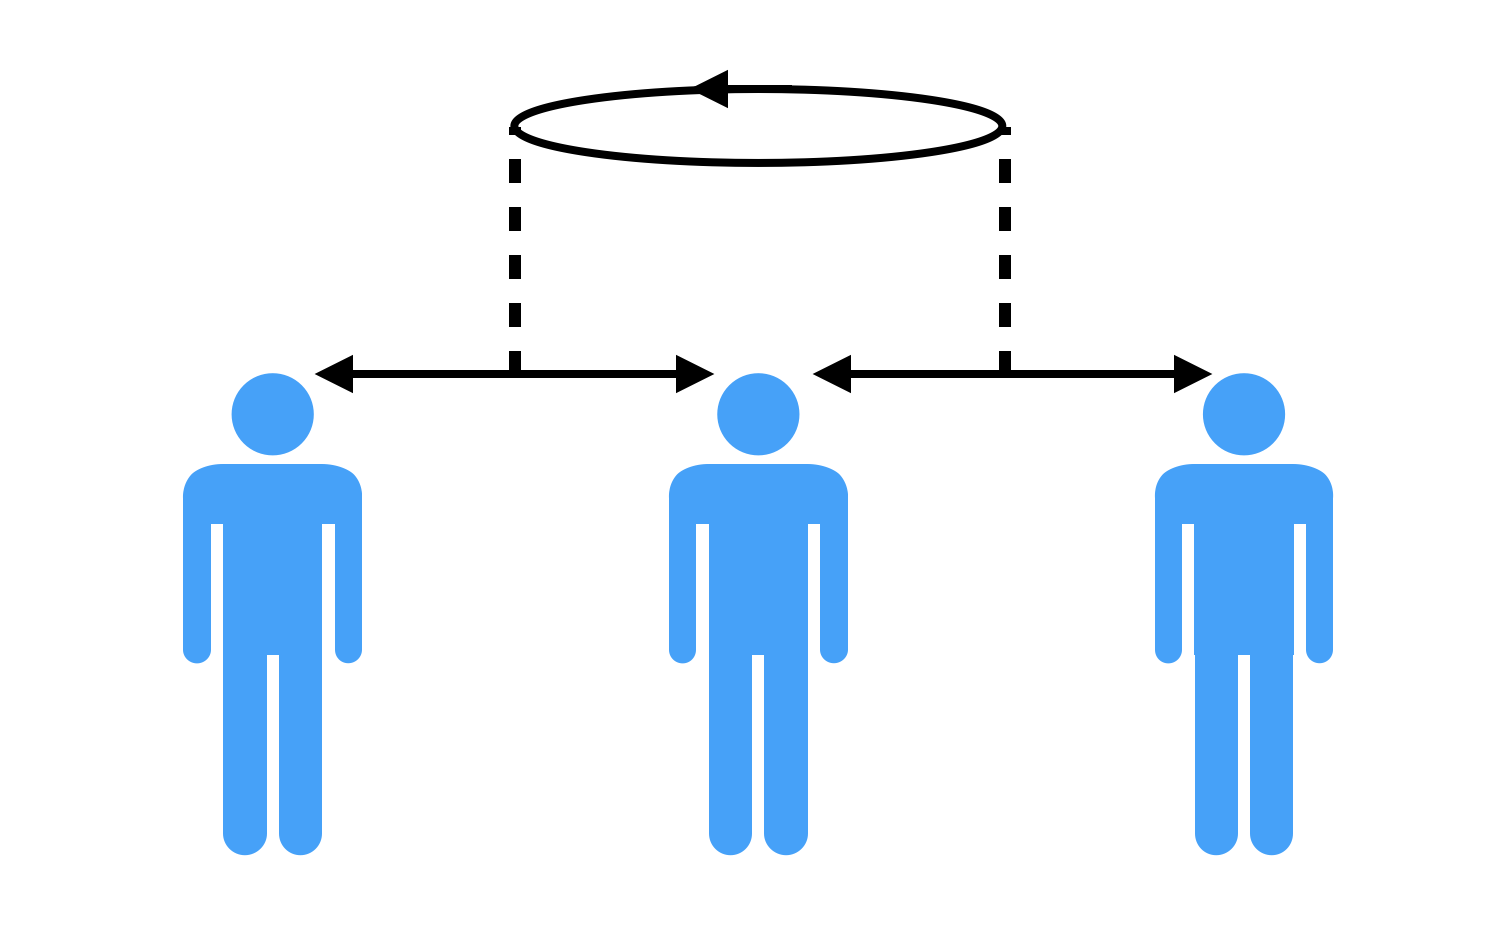
\includegraphics[keepaspectratio,width=0.7\linewidth]{../images/09_Autopoiesis01.png}
	\caption{システムは位相空間\index[termidx]{いそうくうかん@位相空間}に存在する。図中の上でループしているのがシステム。人は要素ではなく，人と人との間にある「関係」のほうが要素}
	\label{Autopoiesis}
\end{figure}

人間の方が添え物ですよ，という話になると，「あれ？生命の話がしたかったんじゃないの?これ生命でしょ?人って生命でしょ?僕もあなたも生命でしょ?」と思うかもしれない。
でも僕はね，「こういう境界があって，こういう物理的な実体があって，それが自分というシステムじゃないか」と思うかもしれませんが，そこに自己はないという考え方です。

なぜなら，この僕の物理的な輪郭や体の境界というのは，外部が観察して境界を決めなければならないものだからです。自分という物理的なものによって，「こすぎ」というシステムは生命を維持してますよ，もちろん。その物理のベースが破壊されたら動かなくなりますが，本質的には，頭の中で考えている認知を，その結びつけ方のネットワークのシステムが，「私」というものです。極端な話，その「こすぎ」の考えていること，つながり方のネットワークが維持されているのであれば，それこそが自己と言っていいんじゃないかというわけです。どうでしょう，ちょっとは伝わったでしょうか。

その物理的な実体というのが，いらないと言っているわけではなくて，この要素関係を要素とするようなシステムのことを論じているのが，オートポイエーシス\index[termidx]{おーとぽいえーしす@オートポイエーシス}だということです。
生命というのは，プロセスの，こういった自分というもの，プロセスのシステムなんだという話をするのです。存在しているのは，物理的な世界ではなくて，位相空間\index[termidx]{いそうくうかん@位相空間}と言ったりします。関係同士を表している位相空間\index[termidx]{いそうくうかん@位相空間}というのは，「実在するもの」なんですよ。それが，オートポイレシスシステムを語る上での重要なポイントです。

そこが十分に語り切れてないので，「入力も出力もない」とかって言われると，「食べてるじゃないか」とか「出してるじゃないか」といった，物理的な生き物としてのインプットとアウトプットを考えてしまうんですね。それは生き物を物理的に定義しているからそういう言い方になるんです。そうではなくて，物理的実体に基盤を置いている，機能的な要素のシステムなんだということが，ポイントです。

\subsubsection{観察者は内側にいる}

そして，もう一つ，二つ目のポイントは何かというと，さっきちょっと触れましたが，観察者の問題です。観察者がシステムに内在化しているということです。
「それがシステムだっていうのは，誰が決めてますか」という問いに対して，外から見て「これがシステム」ですって言ってるんじゃないんです。内側から見て「これが私です」って言ってるんです。「そういうものとして考えられていけないでしょ」って話なんです。

これが難しいんですが，少なくとも，オートポイエシスシステムが言いたかったのはそういうことなんです。「観察者を外に置くと，生命の話ができない」ってことなんです。変なことを言ってるように思えるかもしれませんけど，皆さん確実にわかっていますよね，ほんとはね。「自分が何を考えてるか」っていうことは，自分ではわかりますよね。そして，「他の人が何を考えてるか」っていうのは，決して知り得ない，わかり得ないものなのだということは，絶対皆さんご理解いただいているはずです。

「他の人と気持ちが通じる」とか「心を一つにする」っていうような表現は確かにございます。だけど，「他の人が本当に何を考えているか」なんてのは，絶対にわからないですよね。それは，「他の人」っていうのが，「他の人システム」だからです。そして，「僕」，「私」，「自分」っていうのが，「自分システム」であって，自分システムからは，そのシステムの内側しか見えない。自分の中でしか世界が見えなくなっている，自分の中でしか世界が見えないんです。

だから，どこまで行ったとしても，「あなたのことわかってますよ」っていうのも，「``あなたのことがわかっている''と私は思っています。」ということです。「世界がこうなっていますよ」っていうのは全部，世界がこういうふうになっている「と私は思っていますよ」です。つまり，それは全部，私が主観的に見ている，私という「条件付き」の世界でしかないわけです。

思春期の頃にはえてして，「自分とは何か」っていうのに悩んで，人間というのはどこまで行っても孤独なのだ，「人間というのは最終的には一人なのだ」っていう，独我論に落ち込んでいきがちですよね。哲学的に「自分とは何か」「生きるとは何か」って考える時期があったと思うんです。だけど，だれしもそれを乗り越えて，「人間はどうせ一人だし，どうせ自分の，私の考えるっていう条件は外すことはできないけれども，それを分かった上で少なくとも私はあなたを分かろうとしていますよ」と悟って，努力しないといけない。そうやって社会関係を作っていかないといけないって考えるのが大人ってもんです。そういう人たちが集まって，本質的には分かり得ないけれども，「ここは分かったことにしましょう」っていう共通の理解，共通の社会的な実在性みたいなものをベースに，世の中を作っていくんですよね。

その前提として自分の壁というのは決して超えられないというのがあります。これ，皆さんは分かっているはずです。自分というのが見えているこの世界が，「これが世界ですよ」っていうのがあったとしても，自分はこの世界を内側からでしか，自分の中側からでしか見てないんです。この世界の外側から何か刺激があって，この自分を取り囲んでいる世界の外壁に，外から何か衝撃みたいなのがあったりするかもしれません。外的な刺激というのがあるかもしれないけど，あくまでもそれを内側の壁を通じてでしか見てないんですよね，僕たちは(fig\ref{coupling})。

\begin{figure}[ht]
	\centering
	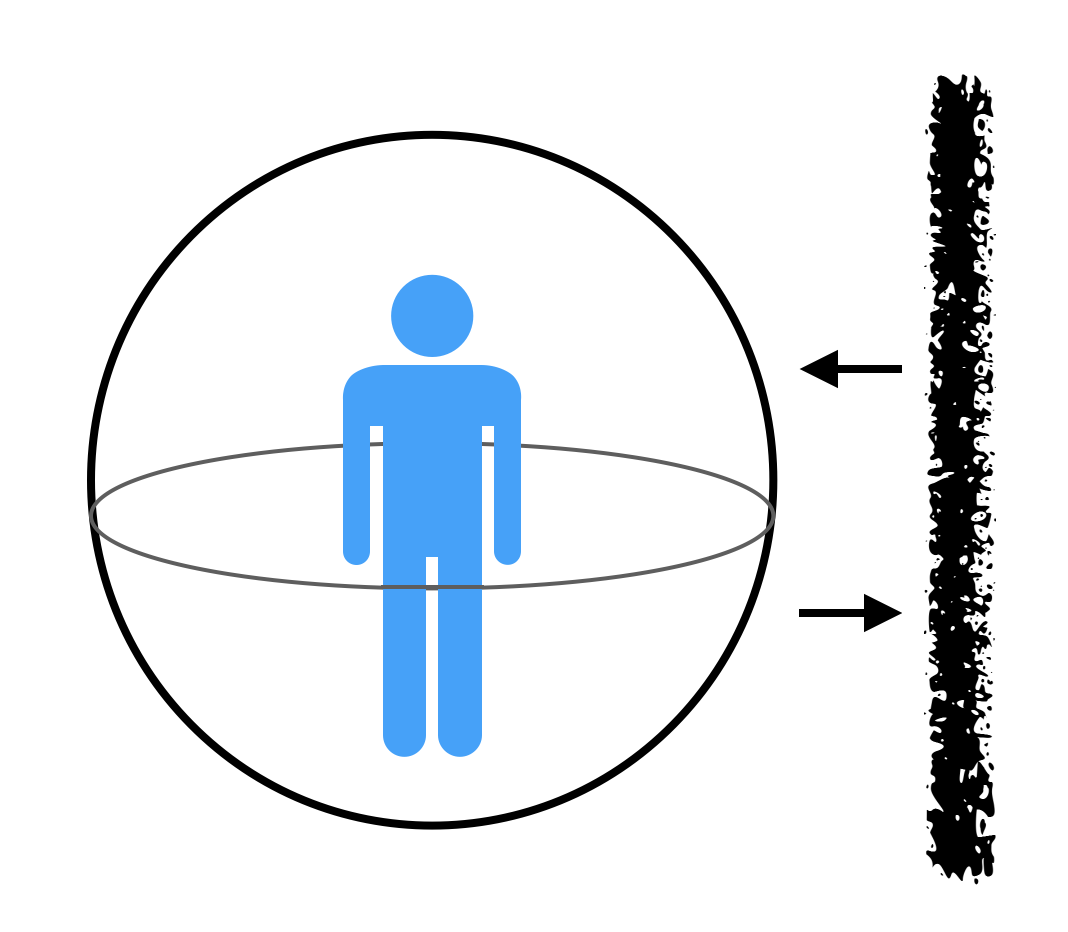
\includegraphics[keepaspectratio,width=0.7\linewidth]{../images/09_cupling.png}
	\caption{システムを内側から見る。外側の外乱はシステムの内側の壁から推察している}
	\label{coupling}
\end{figure}


当たり前の話ですけど，「心理学をやって人の心分かるんですか？」って言われたときに，「分かりますよ」って言ったり，「絶対分かりませんよ」って冗談めかして言います。本当はどっちでもないというかどっちでもいいというか。でもね，「分かるんですか？」って聞いてくる人は，「この自己の壁は絶対破れるはずがないでしょ」っていうのを確信してるはずなんです。答える方も確信してる。だから，そんなことをどう返答しても，どっちでもいいことです。

生命とかシステムとかっていうのを考えるときは，外から見てるのではなくて，この中に入ったものとして捉えないといけないのですよ。中側からシステムを見るので，入出力なんかないんですよ。外からの外壁に何かあるのかもしれないけど，内側の壁に伝わったものを内側から見て，外壁の向こうに何かあったんだろうなと思う。この世界の外側があるんでしょうね，きっとね。あると思っている自己っていうのを，みんな作ってるわけです。生命っていうのはそもそもそういうもんですよってことを，オートポイエーシス\index[termidx]{おーとぽいえーしす@オートポイエーシス}では言っているわけです。

繰り返しですが，心とか私とかっていうシステムの要素は，体のような物理的な実体ではなくて，思考の認知の要素みたいなものだと思ってください。それらの繋がり方が一定のパターンを持ったら，それが自己というものです。頭の中でどのようにそれが繋がっているかというのは，他人の心の中は絶対わかり得ないわけですね。

私も教育者として教育してて，そんな時々思うんですけど，最終的にはもう「分かってくれよ」って言わないうしかないみたいなことって思ったことがありますね。
一生懸命言葉を尽くして喋るんですけど，学習者の側が分かろうとしていなかったら，絶対に理解はしてもらえないですよ。まあ理解したかどうかも，外部からはわからないんですけど。
理解というのは自己の状態，認知の要素のつながりが変わることですから，この人が内側から変化してもらわないと，その人の理解や心の変化につながらないのです。外側からどれだけ働きかけても，内側が変わったかどうかは分かり得ません。もちろん，テストするなどして，反応のパターンを記録し，点数をつけることは可能かもしれません。それにしたって，「私が観測した」とおいう前提条件からは，決して離れられません。オートポイエーシス\index[termidx]{おーとぽいえーしす@オートポイエーシス}も，基本的にこのスタンスで説明しています。入出力が不在。視覚の細胞の反応は外的な環境と別に因果関係を持っているわけではない。神経システムは勝手に発火する，というようなことを言っているのです。

\subsubsection{構造的カップリング\index[termidx]{こうぞうてきかっぷりんぐ@構造的カップリング}}

しかし，それは環境がないというわけではないです。オートポイエーシス\index[termidx]{おーとぽいえーしす@オートポイエーシス}の説明によると，このシステムの外側に環境，あるいは他のシステムが存在します。ここに他人がいた場合，その他人の世界が，壁のあたりを共有しているでしょう。そう考えると，システムはこのような形で成立していると言えます。オートポイエシスは，システムと環境の外部との関係を「構造的にカップリングしている」と表現します。

しかし，この「構造的にカップリングしている」という表現が，具体的に何を意味するのか，私にはわかりません。システムの境界と環境は相互に浸透している，というような言い方をしますが，それが何を指すのかははっきりしないです。私は，システムの外壁が外側の環境と接触していると理解しています。
\begin{figure}[ht]
	\centering
	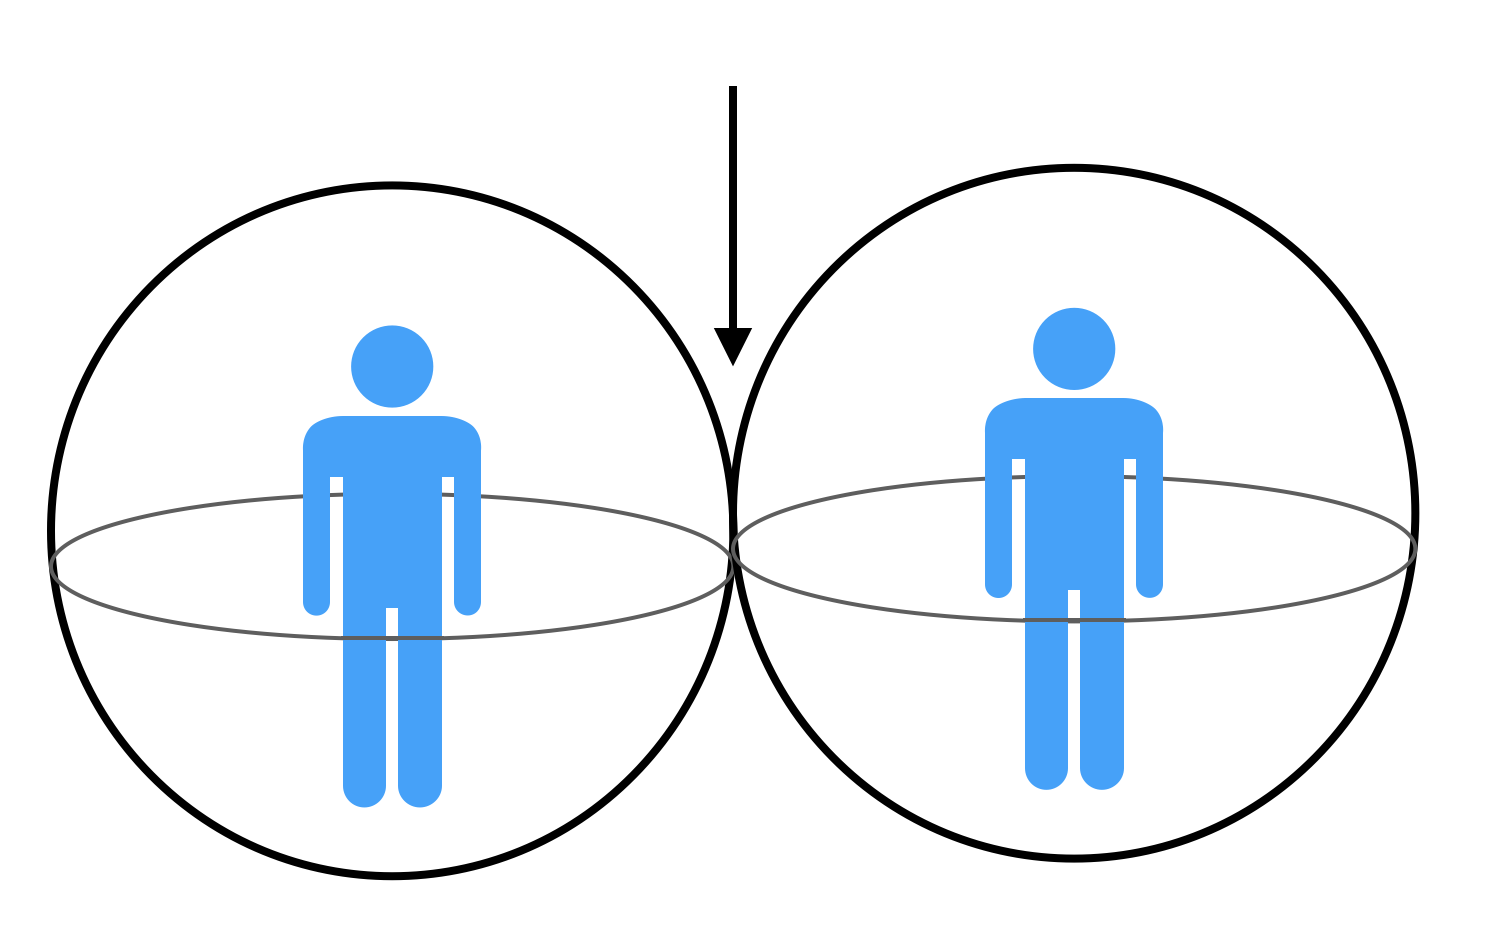
\includegraphics[keepaspectratio,width=0.7\linewidth]{../images/09_coupling2.png}
	\caption{他システムとは境界を接している？}
	\label{coupling2}
\end{figure}

オートポイエシスシステムが解釈しにくいのは，視点が突然システムの中に入ることです。また，物理的なものを観察していた視点ではない。要素の存在性が変わっているということです。ここを違えると，「何だこの話は？」という感じになります。


ルーマン\index[nameidx]{るーまん@ルーマン}は，コミュニケーション\index[termidx]{こみゅにけーしょん@コミュニケーション}が要素であると説明しています。コミュニケーション\index[termidx]{こみゅにけーしょん@コミュニケーション}が相互に関係し合い，その輪が閉じれば，それが社会だという言い方をします。
社会が存在する理由は，複雑性の低減\index[termidx]{ふくざつせいのていげん@複雑性の低減}です。人間がコミュニケーション\index[termidx]{こみゅにけーしょん@コミュニケーション}を行うとき，選択肢は無数にある。その可能性は無限です。しかし，この無限の可能性を試すと，世界は安定せず，複雑極まりないものになります。なので，「ここではこのようなパターンでコミュニケーション\index[termidx]{こみゅにけーしょん@コミュニケーション}を行いましょう」というルールやパターンが必要となります。それをコミュニケーション\index[termidx]{こみゅにけーしょん@コミュニケーション}のスキーマ，スクリプト，パターン，などと言いますが，ともかくある程度の安定した状態を作っている。安定したパターンが作られていることによって，コミュニケーション\index[termidx]{こみゅにけーしょん@コミュニケーション}をするときに，悩む量が随分と減るんですね。例えば，コミュニケーション\index[termidx]{こみゅにけーしょん@コミュニケーション}の仕方がわからない，言語が通じるかどうかもわからない相手がいたとしても，その人がお金を出してきたら，何か売ってほしいんだなということはわかる。そうすることによって，コミュニケーション\index[termidx]{こみゅにけーしょん@コミュニケーション}のパターンが急激に可能性が絞られます。

ルーマン\index[nameidx]{るーまん@ルーマン}に言わせれば，社会というのがなぜあるかというと，それは複雑性を低減するためです。そのとき，社会の要素というのは，コミュニケーション\index[termidx]{こみゅにけーしょん@コミュニケーション}のパターンなんだという説明の仕方をします。これがルーマン\index[nameidx]{るーまん@ルーマン}の社会学における，オートポイエーシス\index[termidx]{おーとぽいえーしす@オートポイエーシス}の導入の仕方です。

社会学者は，社会とは何かを考えることがポイントです。私たちは社会心理学\index[termidx]{しゃかいしんりがく@社会心理学}者ですから，心のことも社会のことも考えなければなりません。そして心のことというのは，思考認知の要素のパターンだと思います。それが一つの，会話のコミュニケーション\index[termidx]{こみゅにけーしょん@コミュニケーション}や生命のパターンを生み出します。その生命のパターンが他の人とネットワークを組み始めると，グループや社会が形成されます。
この思考パターンと他者の思考パターンが，何らかの全体性を形作ったら，そこに新しいシステム，社会，グループが生まれるんですね。これって，レヴィンのライフスペースの発想と同じだと思いませんか。おそらくレヴィンが言おうとしたのは，そういうことだと思います。皆さん，いかがでしょうか。

\section{まとめにかえて}

今言ったようなところが，オートポイエシス論の解釈です。オートポイエシスというシステムがどういう特徴かというと，「自律性」，「個体性」，「境界の自己決定」，「入出力の不在」の4つにつきます。加えて，構造的なカップリングというキーワードが中心かと思います。ただ，彼らの主張するシステムは，生命をどのような観点から捉えるべきかという話が物理的な要素の話をしていないということと，観察者を内側に入れた観点から話しているということが，明示的に語られて指摘されていないため，理解しにくいことがあります。

僕自身，河本の本を何回も読みましたし，マトゥラーナ\index[nameidx]{まとぅらーな@マトゥラーナ}とヴァレラ\index[nameidx]{ゔぁれら@ヴァレラ}の「知恵の樹」\parencite{Chienoki}も読みましたが，観察者が内在化されていることは明示していないですし，オートポイエーシス\index[termidx]{おーとぽいえーしす@オートポイエーシス}を具体例として考えてみようという話のときに，物理的な実体を例に出して語られるので，混乱してしまいます。でも，ここを押さえておけば，大きな迷子にはならないはずです。

もしかすると，僕のオートポイエシスの理解が根本的に間違っているかもしれないので，皆さんもぜひ，この本やマトゥラーナ\index[nameidx]{まとぅらーな@マトゥラーナ}とヴァレラ\index[nameidx]{ゔぁれら@ヴァレラ}のオートポイエシスの本，あるいはこの後紹介しようと思っている藤澤\parencite{fujisawaNetwork}の本を一読して，どういうシステムができているのかを考えてみてください。

この後，オートポイエシス論の限界や今後どうしていくべきかという話もあるのですが，あと5分ではまとめきれませんので，第三世代システム\index[termidx]{だいさんせだいしすてむ@第三世代システム}論についての話をここで終わります。

第二，第三世代のシステムをご紹介しました，というところで止めておきたいと思います。次回は，第四，第五世代のシステムについてお話しします。それをもって，システム論\index[termidx]{しすてむろん@システム論}のお話を閉じたいと思いますので，そのつもりでお待ちください。3，4分早いですが，今日はここまでにしましょう。お疲れ様でした。

\printbibliography[title=引用文献]

\end{document}

